\documentclass[10pt,a4paper]{article}
\usepackage[utf8]{inputenc}
\usepackage{amsmath}
\usepackage{graphicx}



\begin{document}

\begin{titlepage}
\centering



\includegraphics[scale=0.8]{kesla.PNG} \par

\LARGE
\vspace{2cm}
{Göksenin Hande BAYAZIT\par Asena Melisa SARICI\par Özgür YAZICI}


\end{titlepage}

\newpage

\section*{Topology Selection}

\subsection*{Shunt, Series or Compound?}
In the first weekly meeting, we examined the motor specifications and reviewing the EE362 notes, we observed th echaracteristis for shunt, series and compound field connections. Looking at the characteristics provided in \ref{fig:1}, we decided that using a shunt field winding would be better for a more robust voltage with respect to changing current and a more constant speed.  An outstanding advantage of shunt motors is the ease of speed control.  In shunt and seperately excited motors, the field flux is nearly constant. As a result, increased torque must be accompanied by a very nearly proportional increase in armature current and hence by a smal decrease in counter emf $E_{a}$ to allow this increased current through the small armature resistance.  Since counter emf is determined by flux and speed, the speed must drop slightly. The shunt motor has only 6 per cent drop in speed from no load to full load. Starting torque and maximum torque are limited by the armature current that can be successfully commutated.



\begin{figure}[!ht]
\centering
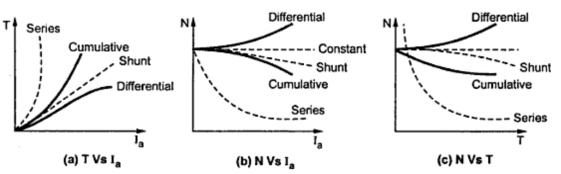
\includegraphics[scale=0.7]{char.jpeg} 
\caption{Characteristics of DC Motor Field Connections}
\label{fig:1}
\end{figure}


\subsection*{Thyristor or Diode?}
To choose the most convenient topology, we compared the advantages and disadvantages of the single phase thyristor rectifier, three phase thyristor rectifier and diode rectifier with buck converter topologies. The results are as follows:

\begin{itemize}
\item Gate driving circuit of a thyristor rectifier is quite hard to implement. Even in the lab experiments, we are not able to set the firing angles precisely. With, diode rectifiers, we will not encounter such a problem.
\item For a three-phase rectifier, 6 thyristors; for a single-phase, 4 thyristors are needed. Considering that for all of these thyristors, there will also be gate driving elements, we will end up with too many number of components, which will cause problems because of debugging, controlling and financial concerns.
\item Thyristor rectifiers work at lower frequency, which causes large ripple.
\item Diode rectifier with buck converter is easier to implement, more affordable and provides more reliable output.
\item As buck converter works at higher frequency, ripple will be quite smaller.

\end{itemize}

\section*{Procedure to be followed for the models}

We decided to make the simulations and the first experiments with a single transistor first(we are every excited about the transistor idea and we will talk about it and we will propose it to professor Ozan Keysan :D). Yet, we aim to design the PCB for an H bridge and continue with our design with H bridge if the first step is successful. Özgür added some MATLAB Simulink simulation which shows the primary model.

\end{document}